% Ch2 slides: conservative form - the flux leaving one cell is exactly the flux entering its neighbour
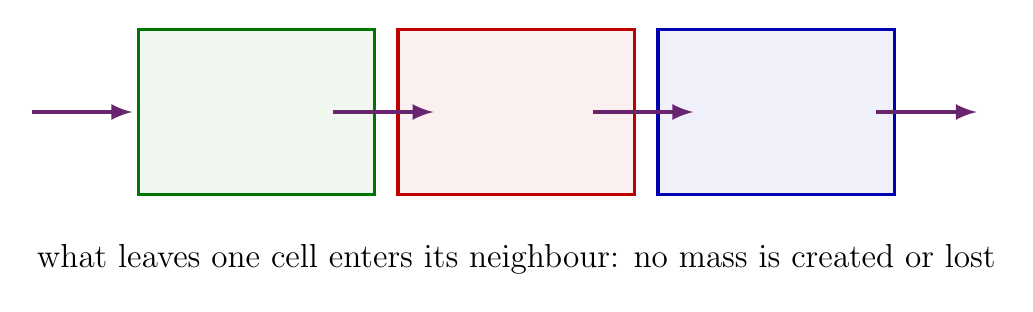
\begin{tikzpicture}[scale=1.5, >=latex]
  \definecolor{dpurple}{HTML}{68246D}
  \foreach \i/\c in {0/green!45!black, 1/red!75!black, 2/blue!70!black} {
    \draw[very thick, \c, fill=\c!6] (2.2*\i,0) rectangle ++(2.0,1.4);
  }
  \foreach \x in {-0.9, 1.65, 3.85, 6.25} \draw[->, ultra thick, dpurple] (\x,0.7) -- ++(0.85,0);
  \node[font=\large, align=center] at (3.2,-0.55) {what leaves one cell enters its neighbour: no mass is created or lost};
\end{tikzpicture}
